% 1985 年全国卷理科第 13 题：两个相交平面及投影关系
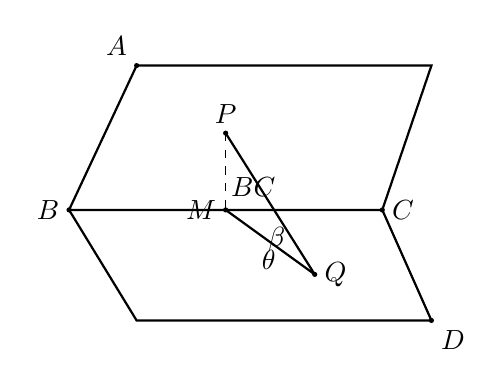
\begin{tikzpicture}[scale=0.78]
  \coordinate (B) at (0,0);
  \coordinate (C) at (5.1,0);
  \coordinate (A) at (1.1,2.35);
  \coordinate (E) at (5.9,2.35);
  \coordinate (F) at (1.1,-1.8);
  \coordinate (D) at (5.9,-1.8);
  \coordinate (P) at (2.55,1.25);
  \coordinate (M) at (2.55,0);
  \coordinate (Q) at (4.0,-1.05);
  \draw[thick] (B)--(A)--(E)--(C)--cycle;
  \draw[thick] (B)--(F)--(D)--(C);
  \draw[thick] (B)--(C);
  \draw[dashed] (P)--(M);
  \draw[thick] (P)--(Q);
  \draw[thick] (M)--(Q);
  \fill (A) circle (1.2pt) node[above left] {$A$};
  \fill (B) circle (1.2pt) node[left] {$B$};
  \fill (C) circle (1.2pt) node[right] {$C$};
  \fill (D) circle (1.2pt) node[below right] {$D$};
  \fill (P) circle (1.2pt) node[above] {$P$};
  \fill (M) circle (1.2pt) node[left] {$M$};
  \fill (Q) circle (1.2pt) node[right] {$Q$};
  \node at (3.0,0.38) {$BC$};
  \node at (3.38,-0.48) {$\beta$};
  \node at (3.25,-0.82) {$\theta$};
\end{tikzpicture}
